% LaTeX layout by Jonas Kahler, jonas@derkahler.de
% HashTux SAD Document
% Group Tux:
% Aman Dirar, Jerker Ersare, Jonas Kahler, Dennis Karlberg
% Niklas le Comte, Marco Trifance, Ivo Vryashkov
% Chapter 7 - Deployment View
\chapter{Deployment View}
These are the components we need to deploy:
\begin{itemize}
  \item Client UI, rendered in a web browser, uses JavaScript
  \item PHP application, executed on an Apache web server
  \item Backend server, written in Erlang, connecting to CouchDB and social
     media APIs
  \item CouchDB Database (External component)
\end{itemize}
The three server-side components could run on three different hosts, which would
result in a four-tier deployment of our components since the client can also be
seen as a tier. \newline
However, we are running the full stack of server-side components on each
physical server node (four in total), so the application could actually run even
if up to three servers are down at any given moment. \\ \\
In addition, we interact with external APIs:
\begin{itemize}
  \item Twitter
  \item Instagram
  \item YouTube
\end{itemize}
So in total, we can say our solution needs at least 5 tiers (Client, Server
(PHP application, backend server, CouchDB), and the three external API servers),
but is currently deployed with a redundancy of servers.
\newpage
\begin{figure}[ht]
  \centering
  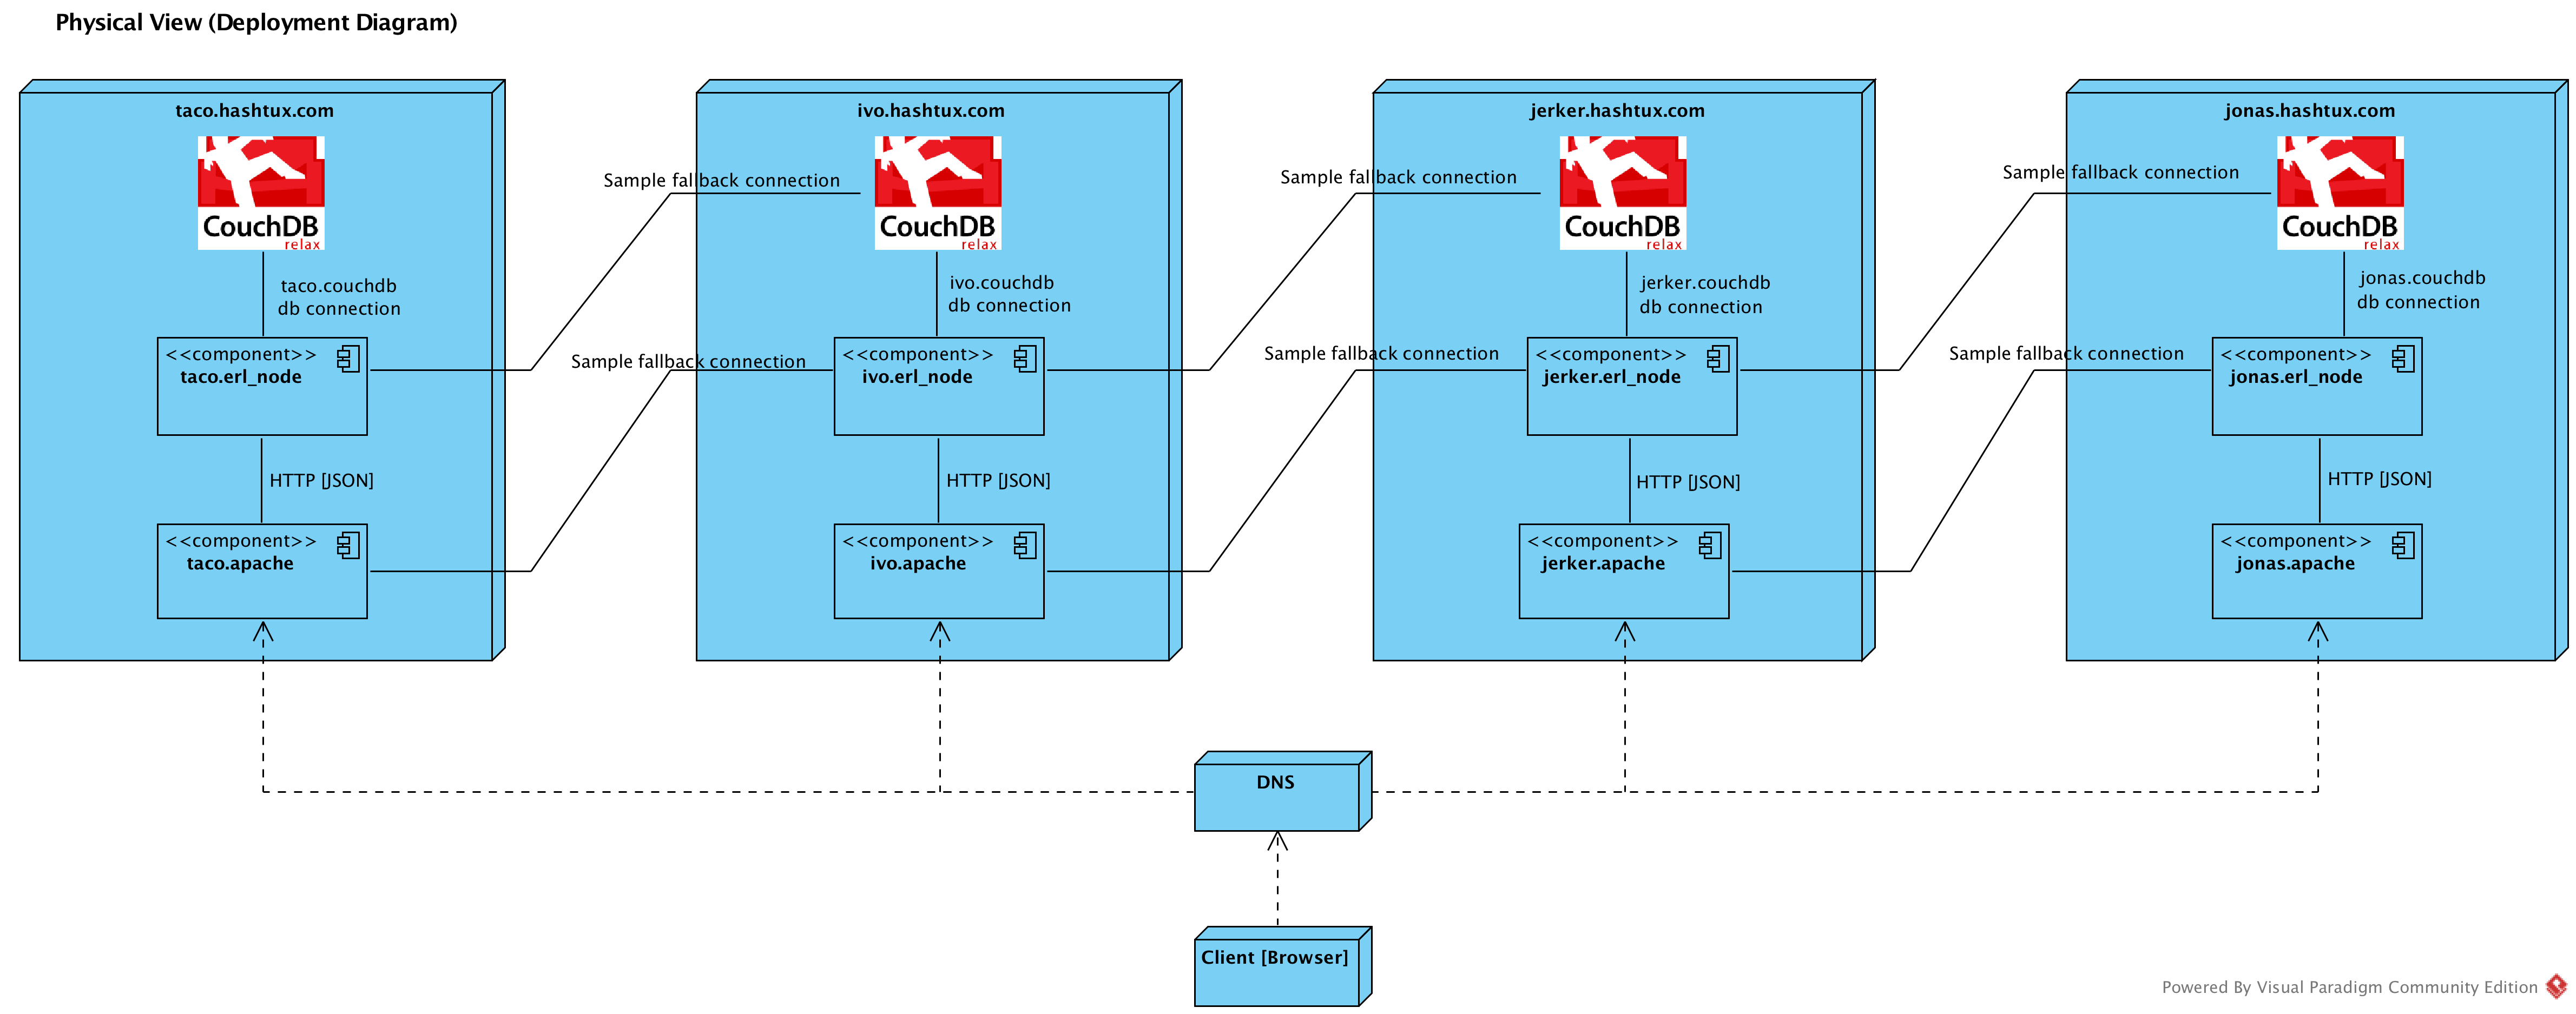
\includegraphics[width=0.6\textwidth]{deployment.png}
  \caption{Deployment Diagram HashTux}
\end{figure}